\documentclass[twocolumn,a4paper]{article}
\usepackage[margin=1in,footskip=0.25in]{geometry}
\providecommand{\keywords}[1]{\textbf{{Keywords: }}#1}
 \usepackage{bibentry} %% to have the publications listed where they are supposed 
\usepackage{comment}
\usepackage[utf8]{inputenc}
\usepackage{graphicx}
\usepackage[numbers]{natbib}
\usepackage{url}
\usepackage[justification=centering]{caption}
\usepackage{authblk}
\newcommand*{\affaddr}[1]{#1} % No op here. Customize it for different styles.
\newcommand*{\affmark}[1][*]{\textsuperscript{#1}}
\newcommand*{\email}[1]{\texttt{#1}}
\usepackage{graphicx}
\graphicspath{ {images/} }
\usepackage[none]{hyphenat}
\usepackage{sectsty}
\allsectionsfont{\centering}


\begin{document}


\title{Automatic Extraction of TEI Structures in Digitized Lexical Resources using Conditional Random Fields}  
\author{%
Mohamed Khemakhem\affmark[1,2,4], {Luca Foppiano\affmark[1] and Laurent Romary\affmark[1,3]\\
\affaddr{\affmark[1]Inria - ALPAGE, Paris}\\
\affaddr{\affmark[2]Centre Marc Bloch, Berlin}\\
\affaddr{\affmark[3]Berlin-Brandenburg Academy of Sciences and Humanities, Berlin}\\
\affaddr{\affmark[4]Université Paris-Diderot, Paris}\\

\email{\{mohamed.khemakhem,luca.foppiano,laurent.romary}\}@inria.fr}\\
}
\maketitle

%\section{Introduction}

\paragraph{}An important number of digitized lexical resources remain unexploited due to their unstructured content.
Manually structuring such resources is a costly task given their multifold complexity. 
Our goal is to find an approach to automatically structure digitized dictionaries, independently from the language or the lexicographic school or style. In this paper we present a first version of \textbf{GROBID-Dictionaries}\footnote{Available at \url{https://github.com/MedKhem/grobid-dictionaries} under the Apache License.}, an open source machine learning system for lexical information extraction.
%\section{Approach}
 
\paragraph{} Our approach is twofold: we perform a cascading structure extraction, while we select at each level specific features for training.

 We followed a ”divide to conquer” strategy to dismantle text constructs in a digitized dictionary, based on the observation of their layout. Main pages (see Figure 1) in almost any dictionary share three blocks: a header (green), a footer (blue) and a body (orange). 
The body is, in its turn, constituted by several entries (red). Each lexical entry can be further decomposed (see Figure 2) as: form (green), etymology (blue), sense (red) or/and related entry. The same logic could be applied further for each extracted block but in the scope of this paper we focus just on the first three levels.
 \begin{figure}
\framebox{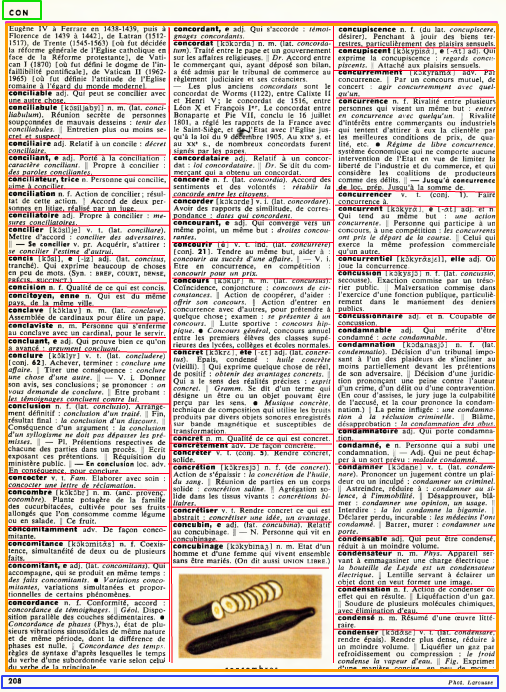
\includegraphics[width=\columnwidth]{larousse-colored.png}} 
\caption{First and second segmentation levels of a dictionary page~\cite{larousse1975france}\label{fig:mouseover}}
%Refering solution according to 
%http://libguides.unitec.ac.nz/apareferencing/images-tables-figures
\end{figure}
\begin{figure}
\framebox{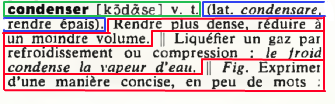
\includegraphics[width=\columnwidth]{larousse-entry-colored-many-senses2.png}} 
\caption{Third segmentation level of a lexical entry~\cite{larousse1975france}\label{fig:mouseover}}
\end{figure}  
 
 The cascading approach ensures a better understanding of the learning process’s output and consequently simplifies the feature selection process. Limited exclusive text blocks per level helps significantly in diagnosing the cause of prediction errors. It allows an early detection and replacement of irrelevant selected features that can bias a trained model. In such a segmentation, it becomes more straightforward to notice that, for instance, the token position in the page is very relevant to detect headers and footers and has almost no pertinence for capturing a sense in a lexical entry which is very often split on two pages.
  




%\section{Grobid \& CRF} 
\paragraph{}To implement our approach, we took up the available infrastructure from GROBID~\cite{Lopez2015GROBIDI}, a machine learning system for the extraction of bibliographic metadata. GROBID adopts the same cascading approach and uses Conditional Random Fields (\textbf{CRF})~\cite{lavergne2010practical} to label text sequences. The output of Grobid dictionary is planned to generate a TEI compliant encoding~\cite{budin2012creating,romary:hal-00704511} where the various segmentation levels are associated with an appropriate XML tessellation. Collaboration with COST ENeL are ongoing to ensure maximal compatibility with existing dictionary projects.
%\section{Experiment and Results}
 
\paragraph{}Our experiments justify so far our choices, where models for the first two levels trained on two different dictionary samples have given a high precision and recall with a small amount of annotated data. Relying mainly on the text layout, we tried to diversify the selected features for each model, on the token and line levels. We are working on tuning features and annotating more data to maintain the good results with new samples and to improve the third segmentation level.

%\section{Related works}
 
\paragraph{}While just few task specific attempts~\cite{bago2015using} have been using machine learning in this research direction, the landscape remains dominated by rule based techniquess~\cite{khemakhem2009towards,fahmy2014towards,mykowiecka2012building} which are ad-hoc and costly, even impossible, to adapt for new lexical resources.
	


\bibliographystyle{plainnat}
\bibliography{Full_Desc}

\end{document}
